% !TeX root = ../main.tex
\section*{Цель работы}
Изучение базовых принципов синтеза работы квадратурного приемника и сравнения его реализаций как на аналоговом принципе, так и на цифровом.

\section{Структурная схема устройства цифровой демодуляции}

На основе исходного кода и классической схемы цифрового квадратурного демодулятора структура моделируемого устройства имеет следующий вид.

\begin{figure}[H]
    \centering
    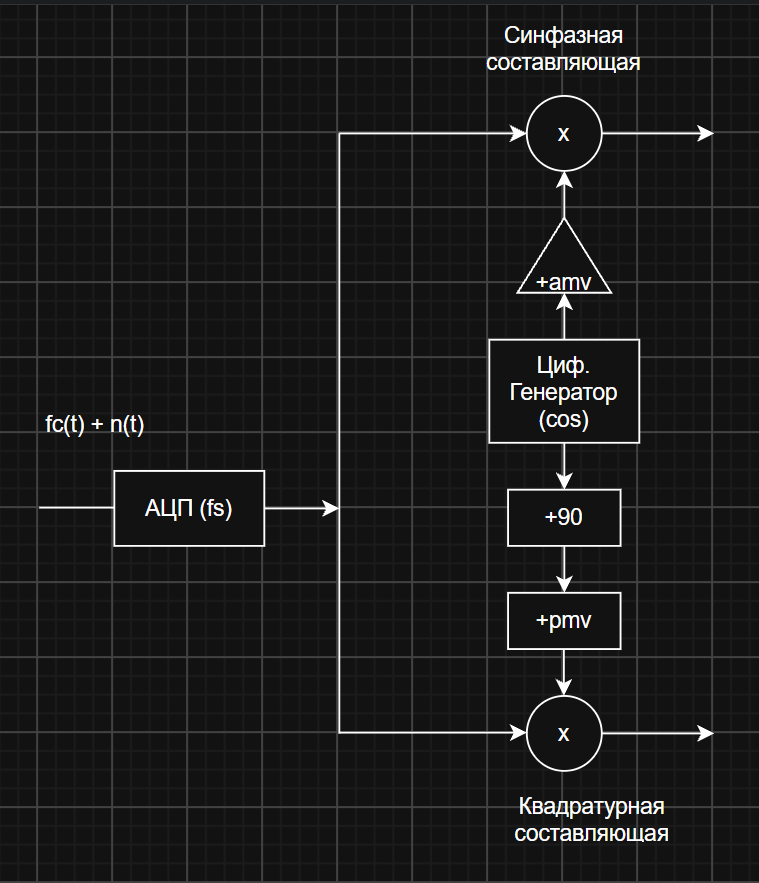
\includegraphics[width=0.8\textwidth]{struc_kod.PNG}
    \caption{Структурная схема работы кода}
\end{figure}

Необходимо заметить, в коде умножение реализовано через комплексные числа: $ dem\_signal = adc\_signal \cdot nco\_signal $, где $nco\_signal$ имеет действительную и мнимую части. Поскольку сигнал с АЦП является вещественным, это математически эквивалентно двум параллельным умножителям, представленным на типовой схеме представленной выше. Фильтры нижних частот (ФНЧ) после перемножителей в данном фрагменте кода не реализованы.


